\section{Analisis Keamanan}
Seluruh pengujian pada bab ini menggunakan blok 64 bit dan 16 putaran, serta dijalankan dengan skrip eksperimen pada repositori menggunakan perintah berikut.

\begin{lstlisting}[basicstyle=\ttfamily\small,breaklines=true]
python3 -m analysis.run_experiments --trials 256 --sample-bytes 4096 --seed 4020 --plots
\end{lstlisting}

Opsi \texttt{--plots} membutuhkan pustaka \texttt{matplotlib}. Skrip menyimpan \textit{seed}, kunci, IV, data mentah setiap percobaan (\texttt{avalanche\_trials.csv}), frekuensi byte (\texttt{histograms.csv}), ringkasan (\texttt{results.json}), dan grafik histogram setiap mode pada direktori \texttt{analysis/results/}, sehingga hasilnya dapat direproduksi.

\subsection{\textit{Avalanche Effect}}
Pada setiap percobaan, dibangkitkan plainteks satu blok, kunci, dan IV secara acak. Kemudian satu bit acak pada plainteks atau pada kunci dibalik, sedangkan masukan lainnya tetap. Persentase \textit{avalanche} dihitung sebagai jumlah bit cipherteks yang berbeda dibagi 64 bit. Blok \textit{padding} PKCS\#7 yang ditambahkan oleh ECB dan CBC tidak ikut dibandingkan, karena blok tersebut tidak bergantung pada bit plainteks yang dibalik dan akan menurunkan persentase secara semu. Hasil 256 percobaan untuk setiap mode ditunjukkan pada Tabel \ref{tab:avalanche}.

\begin{table}[H]
    \centering
    \footnotesize
    \caption{Hasil uji \textit{avalanche effect} (256 percobaan, persentase dari 64 bit)}
    \label{tab:avalanche}
    \begin{tabular}{@{}lcccccccc@{}}
        \toprule
        & \multicolumn{4}{c}{\textbf{1 bit plainteks dibalik}} & \multicolumn{4}{c}{\textbf{1 bit kunci dibalik}} \\
        \cmidrule(lr){2-5} \cmidrule(lr){6-9}
        \textbf{Mode} & \textbf{Rata-rata} & \textbf{Min} & \textbf{Maks} & \textbf{Simp. baku} & \textbf{Rata-rata} & \textbf{Min} & \textbf{Maks} & \textbf{Simp. baku} \\
        \midrule
        ECB & 50,22 & 34,38 & 70,31 & 6,51 & 50,74 & 32,81 & 67,19 & 6,17 \\
        CBC & 50,21 & 31,25 & 67,19 & 6,20 & 49,84 & 34,38 & 65,62 & 6,13 \\
        CFB & 1,56 & 1,56 & 1,56 & 0,00 & 49,54 & 35,94 & 67,19 & 6,12 \\
        OFB & 1,56 & 1,56 & 1,56 & 0,00 & 49,54 & 35,94 & 67,19 & 6,12 \\
        CTR & 1,56 & 1,56 & 1,56 & 0,00 & 49,54 & 35,94 & 67,19 & 6,12 \\
        \bottomrule
    \end{tabular}
\end{table}

Pada ECB dan CBC, perubahan satu bit plainteks mengubah rata-rata sekitar 50\% bit cipherteks, sesuai dengan nilai ideal. Simpangan baku sekitar 6,2\% juga mendekati nilai yang diharapkan apabila setiap bit keluaran berubah secara acak dengan peluang 0,5, yaitu $\sqrt{64 \times 0{,}25}/64 = 6{,}25\%$. Perubahan satu bit kunci menghasilkan sekitar 50\% bit berubah pada kelima mode.

Pada CFB, OFB, dan CTR, perubahan satu bit plainteks hanya mengubah tepat satu bit cipherteks (1,56\% = 1/64). Hal ini merupakan sifat konstruksi mode, bukan kelemahan cipher, karena pada ketiga mode tersebut plainteks hanya di-XOR dengan \textit{keystream}. Nilai uji kunci ketiga mode juga identik karena untuk blok pertama ketiganya menghasilkan \textit{keystream} yang sama, yaitu $E_K(IV)$.

\subsection{Entropi}
Entropi Shannon dihitung dengan $H = -\sum_{x} p(x) \log_2 p(x)$ untuk setiap nilai byte $x$, dengan nilai maksimum 8 bit/byte. Plainteks yang digunakan adalah sampel 4.096 byte berisi byte \texttt{00} sampai \texttt{07} yang diulang, sehingga entropinya tepat 3 bit/byte. Kunci dan IV yang digunakan dibangkitkan dari \textit{seed} 4020, yaitu \texttt{0x34B334ACC96F4286} dan \texttt{0xE6C375B580FD1337}. Hasilnya ditunjukkan pada Tabel \ref{tab:entropi}.

\begin{table}[H]
    \centering
    \small
    \caption{Entropi plainteks dan cipherteks}
    \label{tab:entropi}
    \begin{tabular}{@{}lcc@{}}
        \toprule
        \textbf{Data} & \textbf{Ukuran (byte)} & \textbf{Entropi (bit/byte)} \\
        \midrule
        Plainteks & 4.096 & 3,000 \\
        Cipherteks ECB & 4.104 & 3,020 \\
        Cipherteks CBC & 4.104 & 7,952 \\
        Cipherteks CFB & 4.096 & 7,952 \\
        Cipherteks OFB & 4.096 & 7,949 \\
        Cipherteks CTR & 4.096 & 7,958 \\
        \bottomrule
    \end{tabular}
\end{table}

CBC, CFB, OFB, dan CTR menghasilkan entropi sekitar 7,95 bit/byte. Nilai ini tidak mencapai 8 karena jumlah sampel terbatas. Untuk data acak seragam berukuran sekitar 4.096 byte, nilai harapan entropinya adalah sekitar $8 - 255/(2n \ln 2) \approx 7{,}955$ bit/byte, sehingga hasil keempat mode tersebut setara dengan data acak. Sebaliknya, ECB hanya menghasilkan 3,02 bit/byte. Karena plainteks terdiri atas blok \texttt{00 01 \ldots{} 07} yang berulang, seluruh blok cipherteks ECB juga identik. Hal ini menunjukkan kelemahan ECB dalam menyembunyikan pola, bukan kelemahan cipher.

\subsection{Histogram}
Gambar \ref{fig:hist_ecb} sampai Gambar \ref{fig:hist_ctr} membandingkan frekuensi kemunculan setiap nilai byte pada plainteks (panel atas) dan cipherteks (panel bawah) untuk setiap mode, menggunakan sampel yang sama dengan pengujian entropi.

\begin{figure}[H]
    \centering
    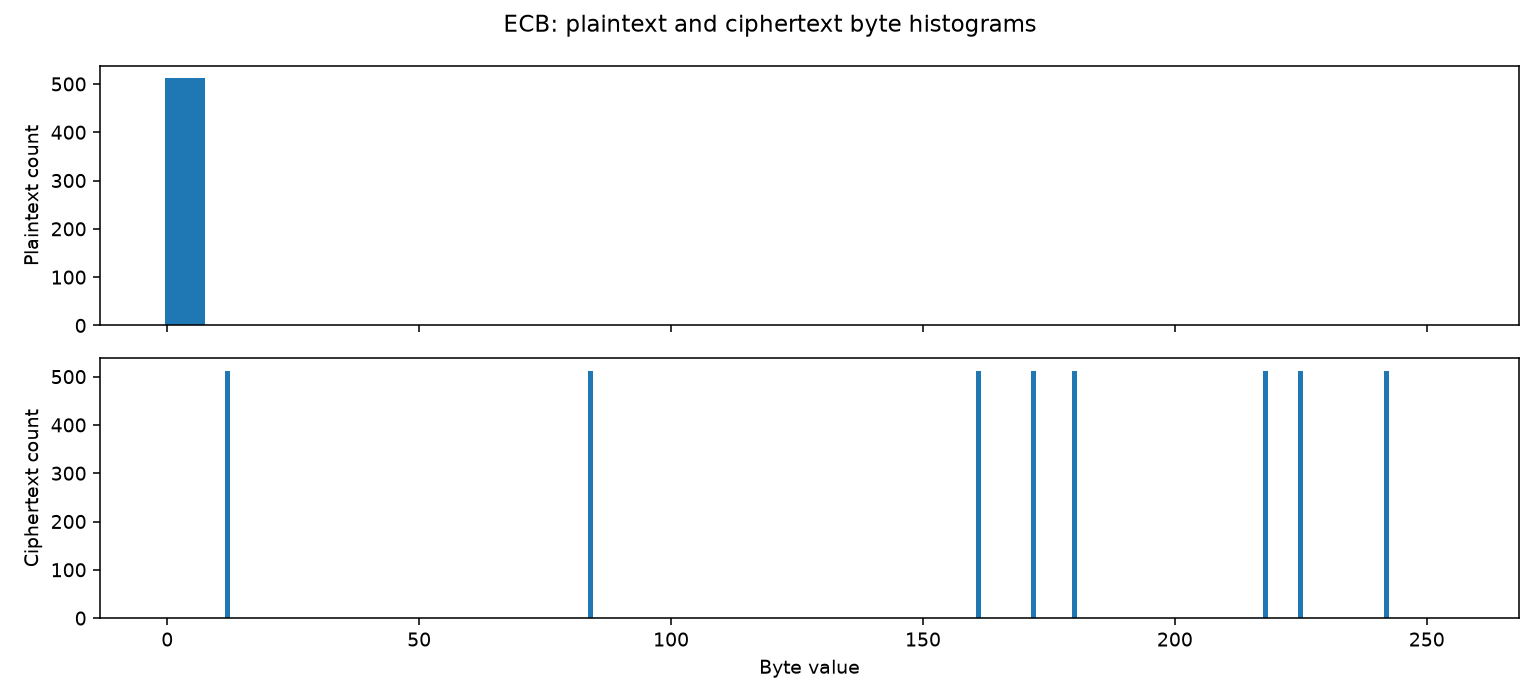
\includegraphics[width=0.9\textwidth]{images/histogram-ecb.png}
    \caption{Histogram byte plainteks dan cipherteks mode ECB}
    \label{fig:hist_ecb}
\end{figure}

\begin{figure}[H]
    \centering
    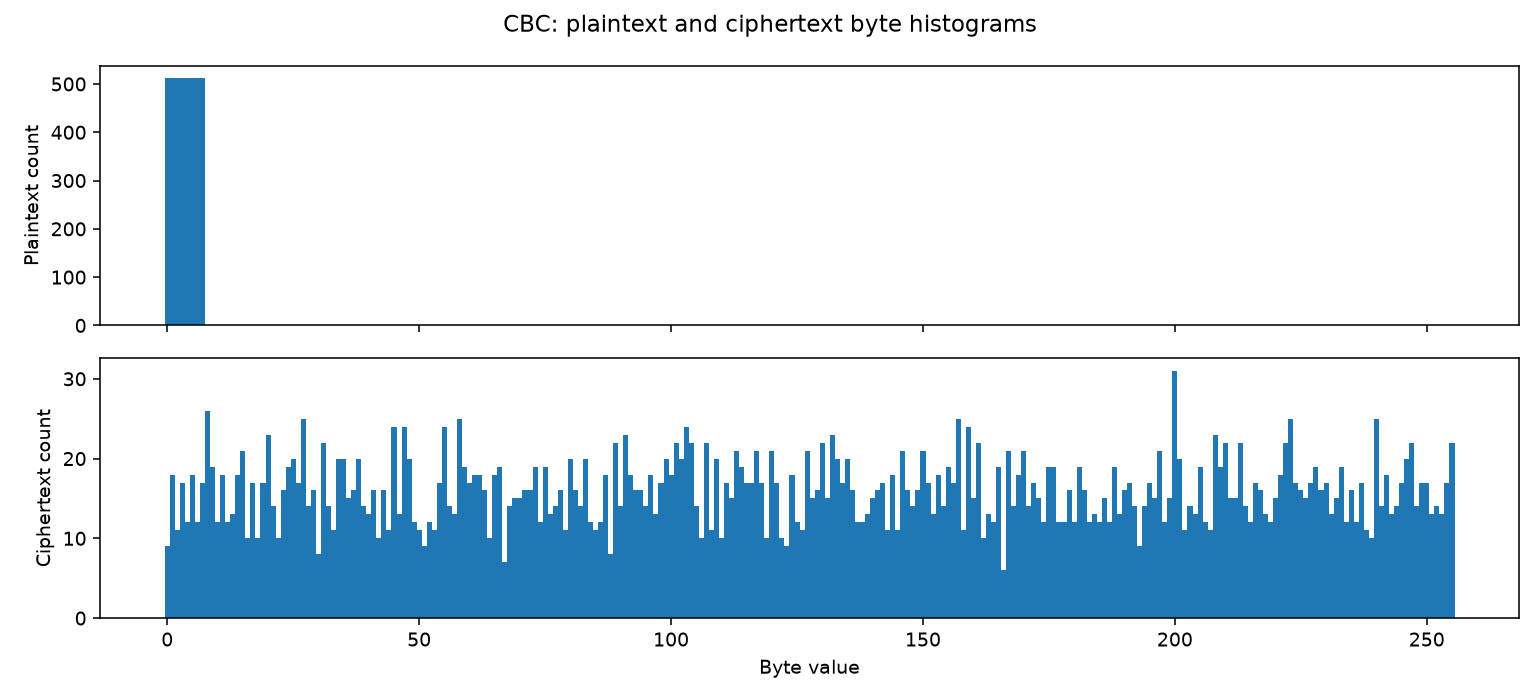
\includegraphics[width=0.9\textwidth]{images/histogram-cbc.png}
    \caption{Histogram byte plainteks dan cipherteks mode CBC}
    \label{fig:hist_cbc}
\end{figure}

\begin{figure}[H]
    \centering
    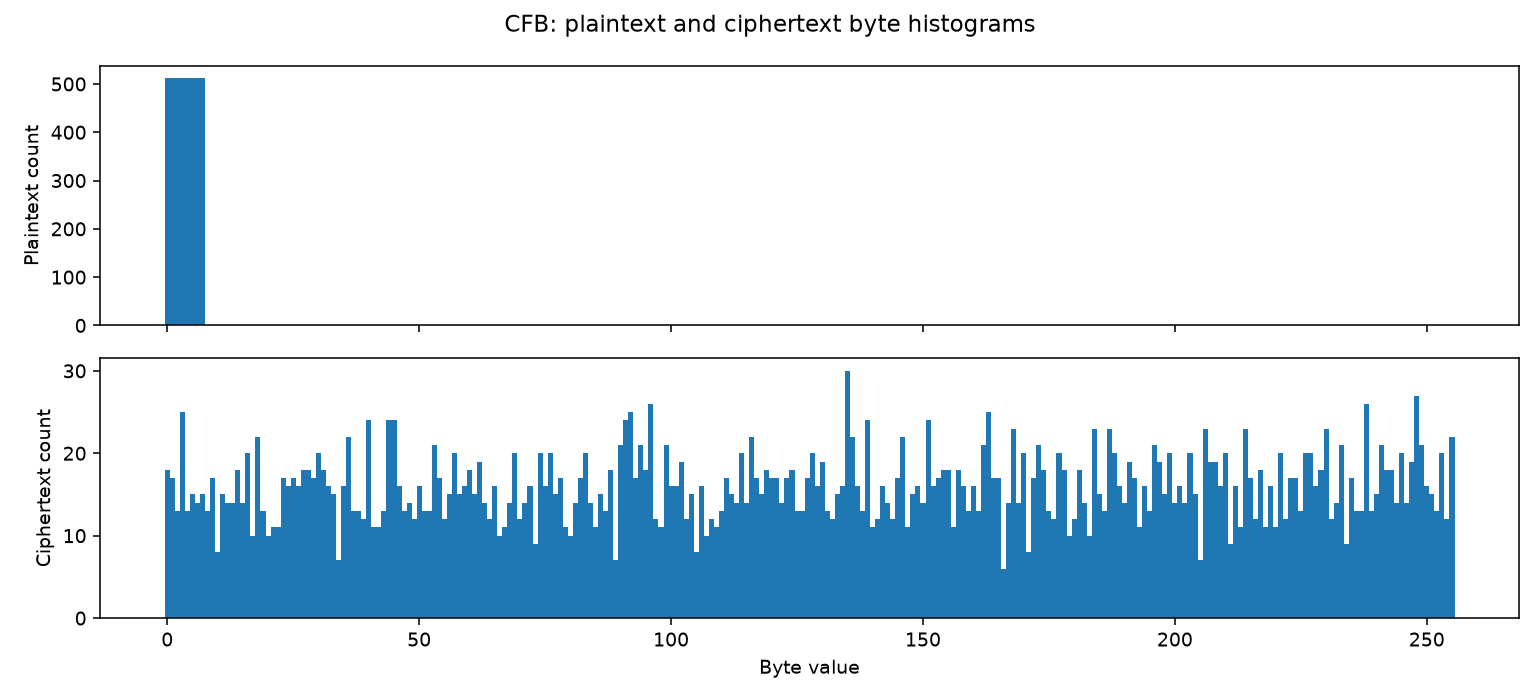
\includegraphics[width=0.9\textwidth]{images/histogram-cfb.png}
    \caption{Histogram byte plainteks dan cipherteks mode CFB}
    \label{fig:hist_cfb}
\end{figure}

\begin{figure}[H]
    \centering
    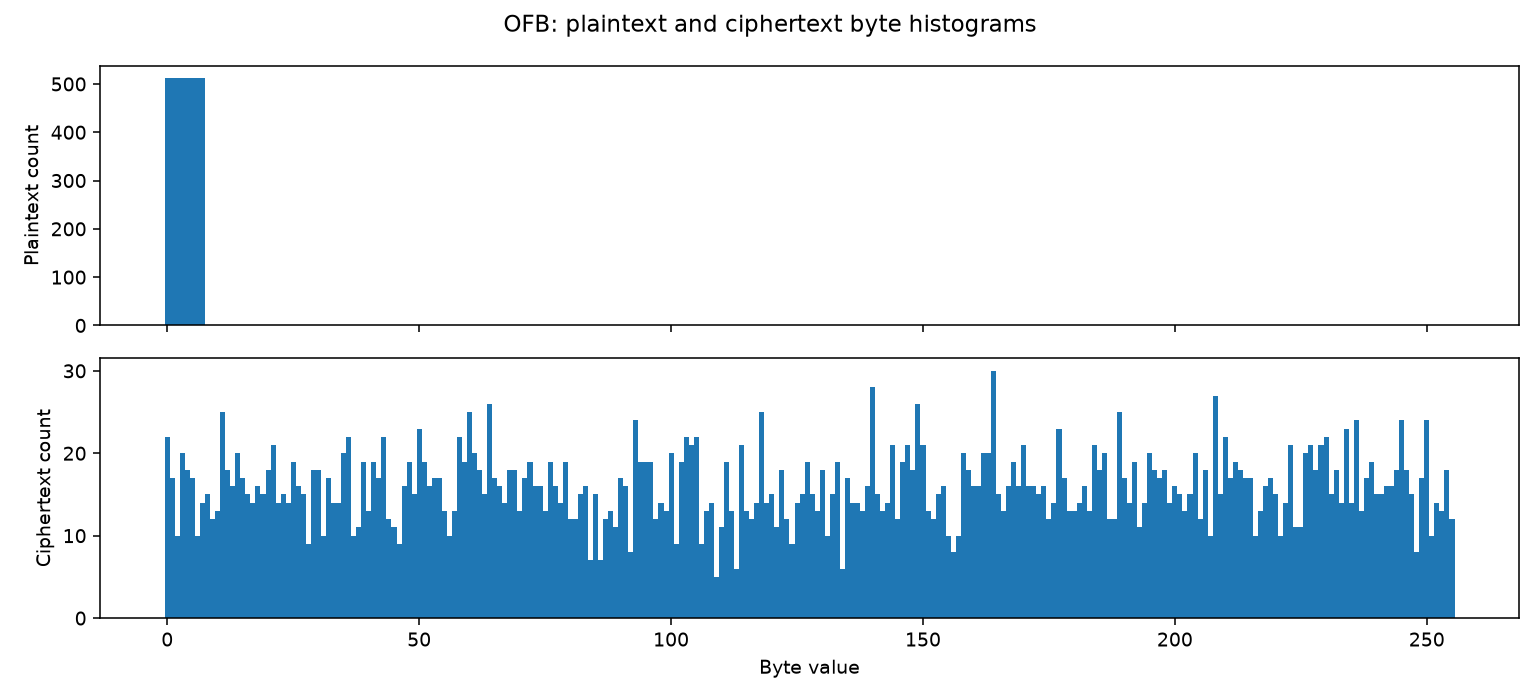
\includegraphics[width=0.9\textwidth]{images/histogram-ofb.png}
    \caption{Histogram byte plainteks dan cipherteks mode OFB}
    \label{fig:hist_ofb}
\end{figure}

\begin{figure}[H]
    \centering
    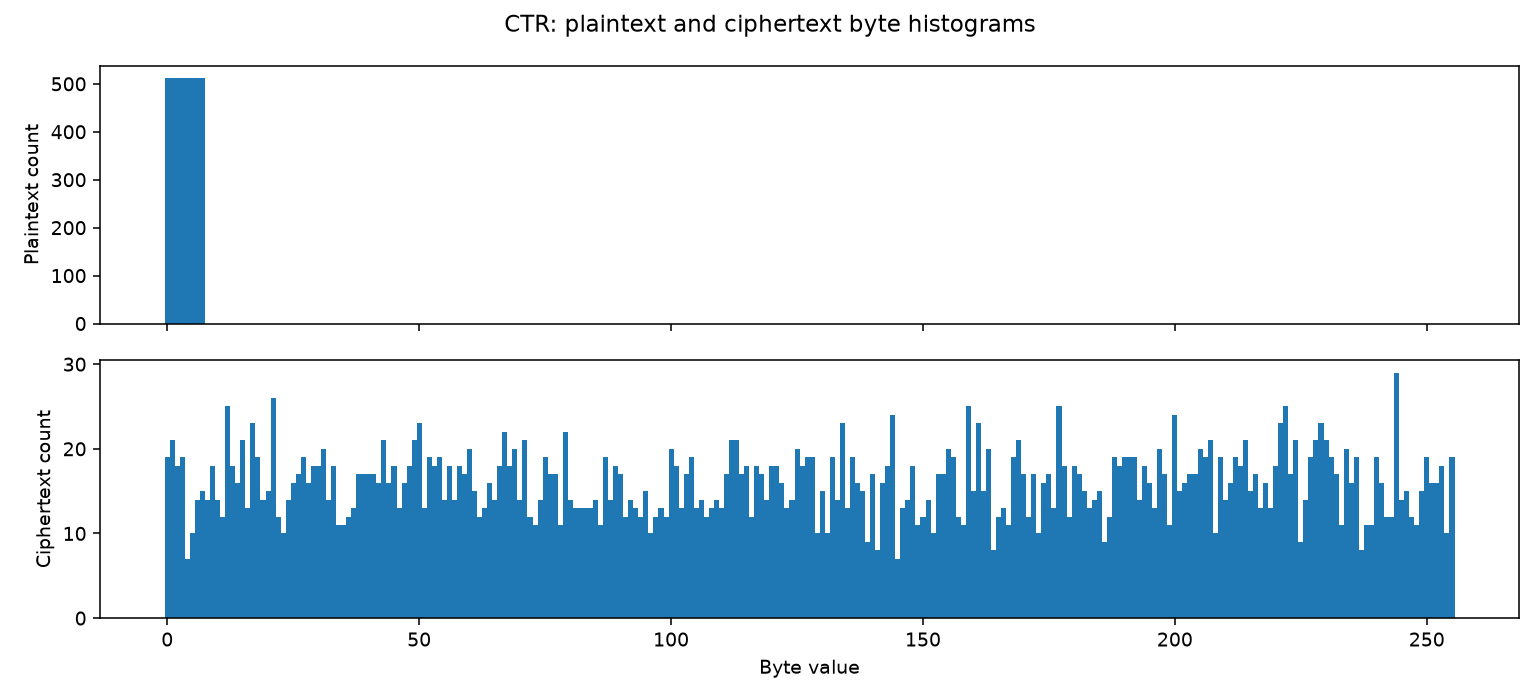
\includegraphics[width=0.9\textwidth]{images/histogram-ctr.png}
    \caption{Histogram byte plainteks dan cipherteks mode CTR}
    \label{fig:hist_ctr}
\end{figure}

Plainteks hanya berisi delapan nilai byte, masing-masing muncul 512 kali. Pada CBC, CFB, OFB, dan CTR, cipherteks tersebar di seluruh rentang 0--255 dengan frekuensi sekitar $4.096/256 = 16$ untuk setiap nilai byte, sehingga distribusinya mendekati seragam dan pola plainteks tidak lagi terlihat. Pada ECB, cipherteks hanya berisi delapan nilai byte dengan frekuensi masing-masing sekitar 512, karena setiap blok plainteks yang identik dienkripsi menjadi blok cipherteks yang identik. Histogram ECB tersebut memperlihatkan secara langsung bahwa ECB membocorkan pola plainteks.

\subsection{Keterbatasan Analisis}
Hasil \textit{avalanche effect} yang mendekati 50\%, entropi yang setara dengan data acak, dan histogram yang mendekati seragam pada mode selain ECB menunjukkan bahwa OATSIDE tidak memiliki kelemahan statistik yang terlihat pada sampel yang diuji. Namun, hasil ini merupakan pengukuran empiris dan tidak membuktikan bahwa OATSIDE aman. Menurutt kami, ada banyak analisis lain yang bisa kita lakukan supaya bisa lebih yakin bahwa OATSIDE aman, misalnya analisis diferensial dan analisis linear. 

\pagebreak
